\begin{figure}[htbp]
    \centering
    \makebox[\textwidth][c]{
        % \begin{tikzpicture}
%     \tikzstyle{every node}=[font=\scriptsize]
%     \definecolor{tabblue}{RGB}{31, 119, 180}
\definecolor{taborange}{RGB}{255, 127, 14}
\definecolor{tabgreen}{RGB}{44, 160, 44}
\definecolor{tabred}{RGB}{214, 39, 40}
\definecolor{tabpurple}{RGB}{148, 103, 189}
\definecolor{tabbrown}{RGB}{140, 86, 75}
\definecolor{tabpink}{RGB}{227, 119, 194}
\definecolor{tabgray}{RGB}{127, 127, 127}
\definecolor{tabolive}{RGB}{188, 189, 34}
\definecolor{tabcyan}{RGB}{23, 190, 207}
\definecolor{ForestGreen}{RGB}{34, 139, 34}
%     \begin{axis}[%
%     hide axis,
%     xmin=10,
%     xmax=50,
%     ymin=0,
%     ymax=0.1,
%     legend style={
%         draw=white!15!black,
%         legend cell align=left,
%         legend columns=3,
%         legend style={
%             draw=none,
%             column sep=1ex,
%             line width=1pt,
%         }
%     },
%     ]

%     \addlegendimage{
%         line legend,
%         tabblue,
%         thick,
%         mark=square*,
%         mark options={line width=1.5pt, rotate=45}
%     }
%     \addlegendentry{\textbf{PEACH Encoder} (Ours)}
%     \addlegendimage{line legend, tabgreen, thick, mark=triangle*, mark options={line width=1.5pt, rotate=0}}
%     \addlegendentry{GNN Encoder}
%     \addlegendimage{
%         line legend,
%         taborange,
%         thick,
%         mark=square*,
%         mark options={line width=1.5pt, rotate=0}
%     }
%     \addlegendentry{PSTNet Encoder}
%     % New Line
%     % \addlegendimage{empty legend}
%     % \addlegendentry{}

%     \addlegendimage{line legend, tabolive, thick, mark=x, mark size=3pt, mark options={line width=1pt}}
%     \addlegendentry{Oracle Encoder}
%     \addlegendimage{line legend, tabcyan, thick, mark=+, mark size=2.5pt, mark options={line width=2pt}}
%     \addlegendentry{MaNGO Mesh Encoder}
%     \addlegendimage{line legend, tabgray, thick, mark=*}
%     \addlegendentry{No Context Encoder}    
%     \end{axis}
% \end{tikzpicture}

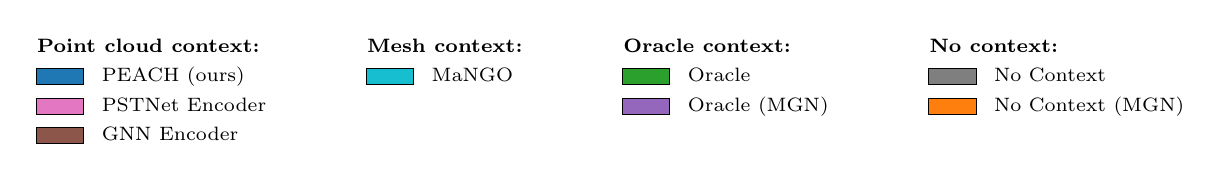
\begin{tikzpicture}
    \tikzstyle{every node}=[font=\scriptsize]
    \definecolor{tabblue}{RGB}{31, 119, 180}
\definecolor{taborange}{RGB}{255, 127, 14}
\definecolor{tabgreen}{RGB}{44, 160, 44}
\definecolor{tabred}{RGB}{214, 39, 40}
\definecolor{tabpurple}{RGB}{148, 103, 189}
\definecolor{tabbrown}{RGB}{140, 86, 75}
\definecolor{tabpink}{RGB}{227, 119, 194}
\definecolor{tabgray}{RGB}{127, 127, 127}
\definecolor{tabolive}{RGB}{188, 189, 34}
\definecolor{tabcyan}{RGB}{23, 190, 207}
\definecolor{ForestGreen}{RGB}{34, 139, 34}
    \begin{axis}[%
        hide axis,
        xmin=10,
        xmax=50,
        ymin=0,
        ymax=0.1,
        legend style={
            draw=none,
            legend cell align=left,
            legend columns=7,
            column sep=1ex,
        }
    ]
        \addlegendimage{area legend, fill=white, draw=white, line width=0pt}
    \addlegendentry{\hspace{-8.2mm}\textbf{Point cloud context:}}
    \addlegendimage{area legend, fill=white, draw=white, line width=0pt}
        \addlegendentry{\hspace{-1ex}}
    \addlegendimage{area legend, fill=white, draw=white, line width=0pt}
    \addlegendentry{\hspace{-8.2mm}\textbf{Mesh context:}}
        \addlegendimage{area legend, fill=white, draw=white, line width=0pt}
        \addlegendentry{\hspace{-1ex}}
    \addlegendimage{area legend, fill=white, draw=white, line width=0pt}
    \addlegendentry{\hspace{-8.2mm}\textbf{Oracle context:}}
        \addlegendimage{area legend, fill=white, draw=white, line width=0pt}
        \addlegendentry{\hspace{-1ex}}
    \addlegendimage{area legend, fill=white, draw=white, line width=0pt}
    \addlegendentry{\hspace{-8.2mm}\textbf{No context:}}
    % Col 1: PEACH
    \addlegendimage{area legend, fill=tabblue}
    \addlegendentry{PEACH (ours)}
    % Col 3: spacer
    \addlegendimage{area legend, fill=white, draw=white, line width=0pt}
    \addlegendentry{\hspace{-1ex}}
    % Col 4: MaNGO
    \addlegendimage{area legend, fill=tabcyan}
    \addlegendentry{MaNGO}
    % Col 5: spacer
    \addlegendimage{area legend, fill=white, draw=white, line width=0pt}
    \addlegendentry{\hspace{-1ex}}
    % Col 6: Oracle + Oracle MGN
    \addlegendimage{area legend, fill=tabgreen}
    \addlegendentry{Oracle}
    % Col 7: spacer
    \addlegendimage{area legend, fill=white, draw=white, line width=0pt}
    \addlegendentry{\hspace{-1ex}}
    % Col 8: No Context + No Context MGN
    \addlegendimage{area legend, fill=tabgray}
    \addlegendentry{No Context}
    % Row 2
        \addlegendimage{area legend, fill=tabpink}
    \addlegendentry{PSTNet Encoder}
    \addlegendimage{area legend, fill=white, draw=white, line width=0pt}
    \addlegendentry{\hspace{-1ex}}
    \addlegendimage{area legend, fill=white, draw=white, line width=0pt}
    \addlegendentry{\hspace{-1ex}}
    \addlegendimage{area legend, fill=white, draw=white, line width=0pt}
    \addlegendentry{\hspace{-1ex}}
    \addlegendimage{area legend, fill=tabpurple}
    \addlegendentry{Oracle (MGN)}
    \addlegendimage{area legend, fill=white, draw=white, line width=0pt}
    \addlegendentry{\hspace{-1ex}}
    \addlegendimage{area legend, fill=taborange}
    \addlegendentry{No Context (MGN)}

        % Col 2: PSTNet
\addlegendimage{area legend, fill=tabbrown}
    \addlegendentry{GNN Encoder}
    \end{axis}
\end{tikzpicture}
    }
    
\includegraphics[width=0.245\textwidth]{figures/quantitative_results/ml_loss_context_line_plots/bbv_context.pdf}\hfill
    
\includegraphics[width=0.245\textwidth]{figures/quantitative_results/ml_loss_context_line_plots/db_context.pdf}\hfill
    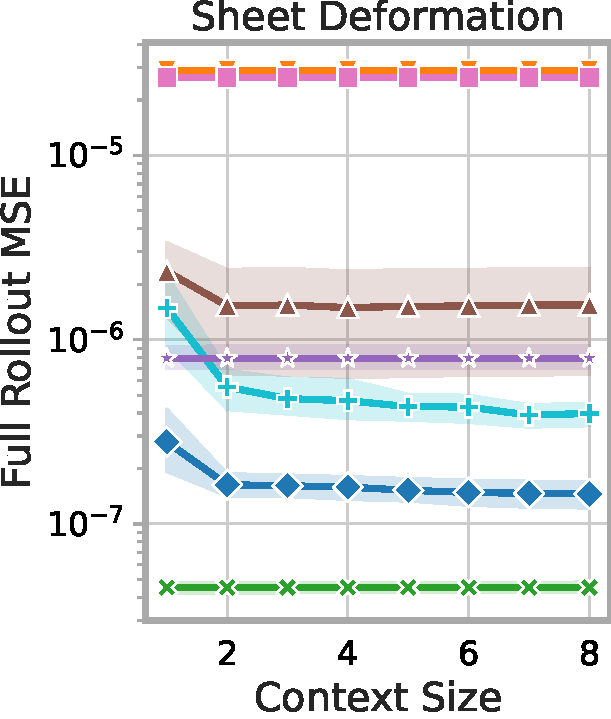
\includegraphics[width=0.245\textwidth]{figures/quantitative_results/ml_loss_context_line_plots/sd_context.pdf}\hfill
    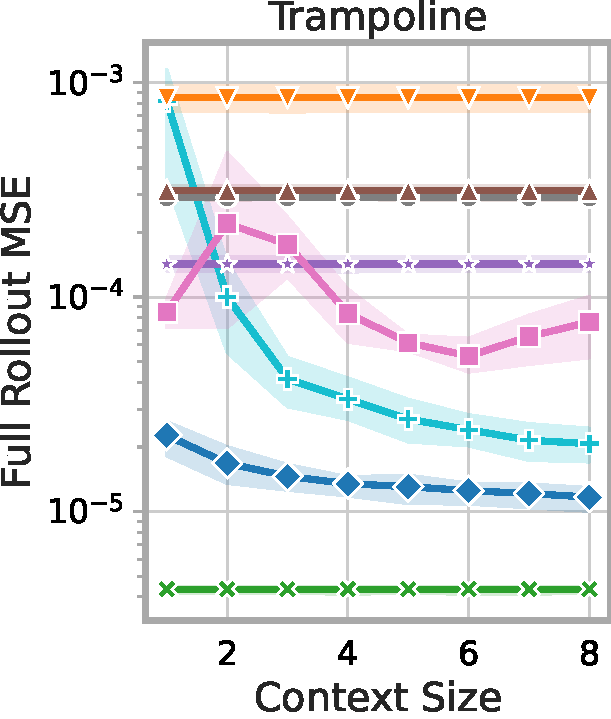
\includegraphics[width=0.245\textwidth]{figures/quantitative_results/ml_loss_context_line_plots/trampoline_v4_sim_context.pdf}
    \caption{Full simulation rollout MSE across different baselines using 8 context trajectories.
    PEACH consistently performs similarly to the mesh-based MaNGO, improving over other
    point cloud-based baselines and achieving performance competitive with the Oracle models.}
    \label{fig:context_mse}
\end{figure}
